

\documentclass[journal]{IEEEtran}

\usepackage{tikz}
\usepackage{pgfplots}
\pgfplotsset{compat=1.18}
\pgfplotsset{hide xscale/.style={/pgfplots/xtick scale label code/.code={}}}
\pgfplotsset{hide yscale/.style={/pgfplots/ytick scale label code/.code={}}}
\usepackage{amsmath}
\usepackage{url}
\hyphenation{op-tical net-works semi-conduc-tor}	% Correct bad hyphenation
\usepackage{graphicx}  % For including figures and pictures
\usepackage{float}  % Used to fix location of images i.e.\begin{figure}[H]
	
\begin{document}

% paper title
\title{Report Title} %\\ \small{Title of the session (you can be creative highlighting your findings)}}

% author names 
\author{Remy Nguyen
    }% <-this % stops a space
        
% Headers
\markboth{National Radio Astronomy Observatory - Domenici Science Operations Center, January 1, 2023}
{Shell \MakeLowercase{\textit{et al.}}: Bare Demo of IEEEtran.cls for IEEE Journals}

\maketitle

% As a general rule, do not put math, special symbols or citations
% in the abstract or keywords.
\begin{abstract}
Provide a summary of the lab session. What was done, 
what measurements were taken, brief methods, what calculations, brief conclusion.  The Abstract should be approximately a few sentences, italicized, in 10-point Times (or Times Roman.) Please leave two spaces between the Abstract and the heading of your first section.
It should briefly summarize the essence of the report and address the following areas without using specific subsection titles. 
\end{abstract}

\begin{IEEEkeywords} %indicate keywords that cover the topic
keywords, temperature, xxxx equation, etc.
\end{IEEEkeywords}

\section{Introduction}
% Here we have the typical use of a "W" for an initial drop letter
% and "RITE" in caps to complete the first word.
% You must have at least 2 lines in the paragraph with the drop letter
% (should never be an issue)

\IEEEPARstart{W}{rite} why it is important to do this experiment, what background is needed, what technology has been used in this session, you can also talk briefly about what other technology exist but was not used here.
Then explain briefly how the experiment was conducted, what measurements were taken, what technology is used (acquisition system, sensors, software), if calculations were done, what calculations were done, what decisions were made, and what the final result was (explained in a concise way with words).
%Objective: Briefly state the problem or issue addressed, in language %accessible to a general scientific audience. Technology or Method: %Briefly summarize the technological innovation or method used to address %the problem. Results: Provide a brief summary of the results and %findings. Conclusions: Give brief concluding remarks on your outcomes. %Detailed discussion of these aspects should be provided in the main body %of the paper.

\subsection{Text and Font}
Normal text is to be single-spaced in 10-point Times or Times Roman (or similar font), with 12-point interline spacing, in the two-column 
format. The first line of each paragraph is to be indented approximately 1/4 inch (approx. 0.7 cm), and the entire text is to be justified -- that is, flush left and flush right. Please do not place additional line spacing between paragraphs. Figure and table captions should be Helvetica 10-point boldface; callouts should be Helvetica 9-point 
nonboldface.  \\

\subsection{Titles and Headings}
The main title should be in Times (or Times Roman) 14-point boldface centered over both columns. In the main title, please initially capitalize nouns, pronouns, verbs, adjectives, and adverbs; do not capitalize articles, coordinate conjunctions, and prepositions (unless the title begins with such a word). Initially capitalize only the first word in first-, second-, and third-order headings. Leave two blank lines before author names(s)/affiliation(s).

\section{Procedure}
List of materials used and how these were used / connected (good opportunity to present block diagrams to show connections).
Use good drafting practice when producing figures, graphs, drawings, or schematics and label them for easy
reference. Include schematics for any circuits. 
If using latex use "~cite" command to cite references~\cite{xbandvla}\cite{solartemp}.

What calculations were done. List and number your equations (Eq.~\ref{equation:force}) to be able to referred them in the text. Equations are centered and the equation numbers are right justified. The equation number is placed in ( ). Be sure that the symbols in your equation have been defined. See example Equation~\ref{equation:force}. 
\begin{equation}
    F = ma
    \label{equation:force}
\end{equation}
Where F equals to force, m to mass and a to acceleration.  

\section{Results}
Show plots of any data collected and describe with words what your plots are showing. Describe the relationship between variables and time. Remember to number all your figures.  This is the most critical part affect the technical achievement.\\
No picture, table, schematic, or graph should appear without a name (generally of the form Fig.1 o Table 1). %~\ref{fig:ecg} or Table~\ref{table:Exps}), 
None should appear without a reference to them by name in the main body of the writing.
All figures and tables must be discussed in the text, including what it is, significant observations, and analysis. \\
Capitalize “Table” and “Fig.” any time they are accompanied by specific table or figure numbers. Examples: “The measured data are plotted in Fig. 2. The figure shows a linear relationship in....”. “The table shows …” vs. “The data of Table 3…” \\

\begin{table}[!ht] %[H]
\centering
\label{table:Exps}
\begin{tabular}{ll}
Student &  Max Temperature \\ \hline
aabbbccc &  $35^{\circ}$   \\
eeeddd &   $54^{\circ}$ \\
eeeddd &   $54^{\circ}$ \\
\end{tabular}
\caption{Temperature measurements performed for session 1.}
\end{table}

%you can use a table generator from here: https://www.tablesgenerator.com/#

Use your word processor to make “real tables” (i.e., boxed in, etc.). Center all tables and include a heading and caption with the appropriate table number below each table. For example, “Table 1: Temperature measurements performed for session 1.” 

Figures must be centered, and the figure number and caption is centered beneath the
figure. For example, “Figure~\ref{fig:ecg}”. 

\begin{figure}[H]%[!ht]
\begin {center}
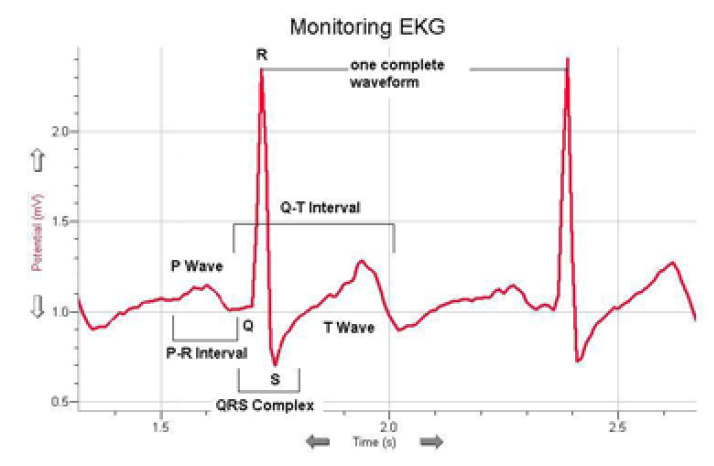
\includegraphics[width=0.45\textwidth]{images/ecg.png}
\caption{Illustrations, graphs, and photographs may fit across both columns, if necessary. Your artwork must be in place in the article.}
\label{fig:ecg}
\end {center}
\end{figure}

\begin{figure}[H]
\begin{tikzpicture}
\begin{axis}[
	title = {Scatterplot Example},
	xmin = 2, xmax = 4,
	ymin = 550, ymax = 700,
	legend pos = north west,
	]
\addplot+[
	only marks,
	scatter,
	mark size=2.9pt
	]
table[meta=B]
{dataplot.txt};
\end{axis}
\end{tikzpicture}
\caption{Scatterplot with imported data}
\label{plot:scatter}
\end{figure}

\begin{figure}[H]
	\begin{tikzpicture}
		\begin{axis}[
			title = {S-Parameter Example},
			grid = both,
			hide xscale,
			xlabel = {Frequency (GHz)},
			enlarge x limits={false},
			xtick distance = 2*10^9,
			scaled x ticks = base 10:-9,
			ymin = 0, 
			ytick distance = 5,
			legend pos = north east,
			]
			\addplot
			table [x = Freq, y = S21, col sep = tab]
			{Amplifier.txt};
		\legend{S21 (dB)	}
		\end{axis}
	\end{tikzpicture}
	\caption{Amplifier S-parameters with imported data}
	\label{plot:graph}
\end{figure}

 Always spell out table or Table. Give abbreviation of Figure, i.e., Fig., when used in
the middle to end of sentence, but spell it out when used at the very start of the
sentence. \\

All graphs must be done with a computer (i.e., spreadsheet software such as
Microsoft Excel or even MATLAB.). Do not include hand drawn graphs unless
specifically instructed to do so.  \\
Include a leading zero when a number’s magnitude is less than 1 (use 0.83 instead of
writing .83). \\
Use your word processor for Greek symbols for common engineering quantities as $\beta$, $\pi$, $\gamma$ ,$\Omega$ . 

\section{Discussion}
Interpretation of results. Discuss any interesting result related to the materials used or to any claim from the introduction. Discuss your measurements using engineering terms (accuracy, precision, resolution, etc).  

\subsection{Subsection}
Use subsections to improve readability.

\section {Conclusions}
What was learned and what recommendations do you have. Give technical conclusions. Restate the main objectives and how or to what degree they were achieved. What principles, laws and/or theory
were validated by the experiment? You can respond to the questions to consider.

% if have a single appendix:
%\appendix[Proof of the Zonklar Equations]
% or
%\appendix  % for no appendix heading
% do not use \section anymore after \appendix, only \section*
% is possibly needed

% use \appendices with more than one appendix
% then use \section to start each appendix
% you must declare a \section before using any
% \subsection or using \label (\appendices by itself
% starts a section numbered zero.)

\appendix
\bibliographystyle{IEEEtran}
\bibliography{references}

\end{document}


